\chapter{Introdução}

\section{Apresentação}

Reconhecimento de gestos baseado em visão computacional é um assunto bastante pesquisado e já pode ser considerado popular, isto porque, a busca por mecanismos que tornem a interação entre homem e máquina mais intuitiva e natural é constante e vem aumentando com o lançamento de plataformas que auxiliam os desenvolvedores nos complexos algoritmos que envolvem essa área.
O lançamento do Kinect, da Microsoft \cite{kinect}, e da plataforma de desenvolvimento da Intel, chamada Intel Perceptual Computing \cite{intel} (figura \ref{fig:depth_camera}),  ambas com câmeras de profundidade, vem popularizando o desenvolvimento de aplicativos e revolucionando o jeito que interagimos com os jogos e computadores. 

\begin{figure}[ht!]
\centering
\fbox{
  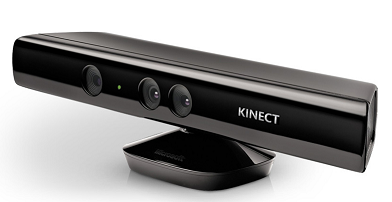
\includegraphics[width=0.3\textwidth]{image/kinect_camera.png}
  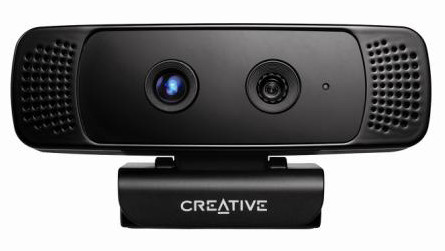
\includegraphics[width=0.3\textwidth]{image/intel_creative_camera.jpg}}
  \caption{Kinect, da Microsoft, e a câmera da \textit{Creative} com parceria da Intel}
  \label{fig:depth_camera}
\end{figure}

O uso de câmeras em carros e caminhões também tem aumentando nos últimos anos. Sistemas de segurança capazes de verificar se o motorista esta saindo indevidamente da faixa, ou se o veículo esta em rota de colisão com algum outro automóvel ou objeto e até mesmo monitorando o stress do motorista já são comuns em vários modelos de veículos. Mas pouco vimos o uso dessas câmeras para interação do motorista com a grande quantidade de controles que temos nos carros. Sistemas de navegação, componentes de som e imagem como CD/DVD player, radio, televisão, celulares, computador de bordo, e ar condicionado são alguns exemplos de dispositivos que requerer uma constante interação com o motorista e cujo comandos poderiam ser dados por meio de gestos.
O sistema de gestos também pode ser usado como um complemento ao sistema de reconhecimento de voz, bastante comum hoje nos carros.

Os gestos e poses, em nossa aplicação, podem ser entendidos como movimentos ou poses executados pela mão direta do motorista dentro do campo de visão de uma câmera instalada no teto do carro.
O nosso estudo, portanto, é focado no histograma orientado a gradientes (HOG - Histogram of oriented gradients) aplicado em um sistema de interface de usuário através de gestos. Um sistema em tempo real capaz de reconhecer poses de mão e gestos que permita o motorista interagir com o veículo de forma intuitiva e eficaz.

\todo {Colocar uma foto do angulo de visão da câmera na nossa aplicação.}

\section{Objetivo}

O objetivo do trabalho é estudar o efeito da variação dos principais parâmetros do cálculo do HOG e assim encontrar qual a melhor configuração para a aplicação proposta. Um balanço entre performance e processamento deve ser levado em consideração, já que o trabalho computacional deve ser reduzido ao máximo para aplicações automotivas.
Em \cite{dalal} foi feito um trabalho parecido para encontrar o melhor conjunto de parâmetros para a representação de seres humanos em diversas situações e poses diferentes. O que queremos avaliar é se para a nossa aplicação, os mesmos parâmetros podem ser aplicados e qual seria o custo na performance do algoritmo se o mesmo fosse simplificado com o intuito de reduzir processamento.
O HOG poderia ser usado de duas maneiras diferentes: como um pre classificador para encontrar as regiões mais prováveis de se ter uma mão e assim limitar a imagem em algumas regiões de interesse aonde um segundo algoritmo seria aplicado, nesse caso não seria trabalho do HOG dizer qual é a pose, mas sim se é uma mão ou não, ou no máximo classificar a pose em algum grupo de poses (como feito em \cite{ref10}). Mas o HOG poderia ser usado também para dizer qual pose é, sem a necessidade de nenhum algoritmo secundário.
Visando que temos duas aplicações para o HOG, é possível que teremos duas configurações diferentes e portanto essas variações devem entrar no escopo desse trabalho.

\section{Justificativa}

A função principal do motorista deve ser sempre controlar o carro e distrações, como operar o rádio ou a central multimédia, deve ser reduzidas ao máximo. Portanto apenas alguns poucos e curtos momentos podem ser usados para interagir com os comandos do veículo. Em estudos de usabilidade, o controle gestual provou ser mais intuitivo, efetivo \cite{ref12}  \cite{ref13} e distrair menos do que o uso habitual de botões \cite{ref14}. Por esse motivo, um estudo sobre técnicas para atingir esse objetivo é justificável.

As condições gerais dentro do automóvel inclui uma grande variação de iluminação, mudança de usuário (cor de pele, braço com ou sem vestimentas e vestimentas de cores e estampas diferentes) e fundos não uniformes. Além disso, a aceitação do usuário é um item bastante importante, portanto coisas como uma iluminação artificial visível, restrição de vestimentas e calibração extensiva não pode ser tolerados. Tento isso em mente, alguns critérios e requisitos para o sistema podem ser estabelecidos:

\begin{itemize}
\item robustez contra ambientes ruidosos
\item iluminação invisível
\item independente de usuário
\item sem calibração ou treinamento pelo usuário
\item pequeno e compreensível conjunto de gestos
\item reação do sistema com o mínimo de latência
\end{itemize}

Em 2005, Navneet Dalal fez um estudo sobre histogramas orientado a gradientes aplicado à detecção de humanos \cite{dalal}. Seu estudo, variando cada parâmetro do cálculo dos histogramas e encontrando um conjunto de parâmetros que melhor servia para reconhecimento de humanos, virou referência para todos os estudos posteriores de HOG. Em seu texto ele diz que o uso de histogramas orientados tem muitos precursores (\todo{Adicionar ref}), mas que apenas atingiu a maturidade quando combinado com histogramas locais e normalização proposto pela Lowes Scale Invariant Feature Transformation (SIFT) (\todo{Adicionar ref}). A conclusão que ele chegou foi que usando histogramas de gradientes locais normalizados, similar ao SIFT, em um grade com sobreposição tem ótimos resultados para detecção de humanos, reduzindo falsos positivos em mais de uma ordem de magnitude comparado com Haar wavelets.

\todo {Pesquisar as principais diferenças entre SIFT e HOG}

% % % % % % % % % % % % % % % % % % % % % % % % % % % % % % % %
% Gesture Components for Natural Interaction with In-Car devices &
% Gesture control for use in auto-mobiles
Em \cite{ref2} (Alemanha, 2000) e em \cite{ref1} (Alemanha, 2003)temos um cenário idêntico ao proposto, onde imagens infra vermelhas de uma câmera instalada no teto do carro são capturadas e traduzidas em gestos e poses de mão. Em \cite{ref1} o sistema proposto pelo artigo é capaz de reconhecer onze gestos e quatro poses. A imagem capturada em uma taxa de 25 fps e resolução 384x144 é primeiramente processada com uma combinação de subtração de fundo e threshold global. Em \cite{ref2} é usado apenas um threshold global. A mão é considerada o maior objeto da cena. Depois da segmentação, um filtro para retirar o braço é aplicado e finalmente são calculados os momentos da imagem, para o cálculo da área e do centro de massa, e os momentos Hu.

% % % % % % % % % % % % % % % % % % % % % % % % % % % % % % % %
% Histograms of Oriented Gradients for Human Detection

% % % % % % % % % % % % % % % % % % % % % % % % % % % % % % % %
% Real-time Vision-based Infotainment User Determination for Driver Assistance
Em \cite{ref5} (Estados Unidos, 2008) temos também o uso de câmera infra vermelha no teto do carro, mas com o objetivo de discriminar qual pessoa está usando o painel de controles do carro, o motorista ou o passageiro. O sistema faz uso do HOG para descrever a imagem e um classificador SVM com uma taxa de 96.8\% de acerto. O cálculo do HOG é uma versão simplificada feita por \cite{dalal}. Nesse artigo, depois de calculado o gradiente da imagem, a mesma é dividida em uma grade de células 2x2, o histograma é calculado para cada célula com 8 bins variando de 0 à 360 graus, portanto formando um vetor de 32 dimensões.

% % % % % % % % % % % % % % % % % % % % % % % % % % % % % % % %
% An Effective Crossing Cyclist Detection on a Moving Vehicle 
Em \cite{ref6} (China, 2010) o HOG é utilizado para detectar ciclistas. No método proposto não é feito overlap no cálculo dos histogramas, como uma maneira de melhorar o tempo de processamento, e amostragem piramidal é utilizada para extrair características globais em diferentes escalas. As imagens utilizadas são em tons de cinza e um filtro gaussiano é aplicado antes do cálculo dos HOGs (contrariando as orientações do Dalal em \cite{dalal}). O gradiente é calculado com máscara [-1 0 +1], os ângulos são calculados entre 0 e 180, e o histograma é dividido em 20 bins. A imagem é dividida em blocos de 16x16 sem divisão de células. O classificador utilizado é um SVM linear. Esse trabalho é interessante pois propõe um método para melhorar a velocidade do cálculo dos histogramas, o que pode ser útil para aplicações em tempo real embarcadas.

% % % % % % % % % % % % % % % % % % % % % % % % % % % % % % % %
% Hand-gesture recognition: comparative study of global, semi-local and local approaches
Um estudo comparando descritores locais, semi locais e globais é feito em \cite{ref7} (França, 2011). O objetivo do trabalho é estudar qual seria o método mais adequado para descrever poses de mão em uma sala de cirurgia para que o médico possa enviar comandos para os aparelhos sem precisa encostar neles. Para descritores globais foi usado os momentos de Zernike (invariante em rotação, translação e escala) combinados com um classificador linear SVM. O HOG é usado como um descritor semi local e SIFT para locais. Apesar de não dar detalhes de como é feito os cálculos do HOG, o artigo mostra uma melhor performance do método.

% % % % % % % % % % % % % % % % % % % % % % % % % % % % % % % %
% A vision-based system for automatic hand washing quality assessment
Nesse artigo \cite{ref16} (Espanha, 2011), o problema a ser resolvido era verificar, com o uso de uma câmera, se uma pessoa  fez as seis diferentes poses de mão para o lavar correto das mãos. Primeiro as imagens são segmentadas por cor de pele e depois um estimador de posição do braço e da mão baseado em um filtro multi modal probabilístico é proposto. Um ROI é criado com o resultado do filtro e anterior e então HOG é aplicado, usando como classificador dois SVM independentes. Uma para o HOG normal e outro para o HOF (Histogram of optical flow).

% % % % % % % % % % % % % % % % % % % % % % % % % % % % % % % %
% Automatic Ship Recognition Robust Against Aspect Angle Changes and Occlusions
Nesse artigo \cite{ref8} (Japão, 2012), é utilizado a coHOG (co-occurence HOG) para reconhecimento de navios em imagens ISAR. No coHOG os blocos são agrupados em pares, aumentado a robustez para imagens em diferentes ângulos e na oclusão de algumas partes do navio. Por outro lado, o coHOG tem uma alta dimensão.

% An Extended HOG Model: SCHOG for Human Hand Detection
% 2012 / China
% [1, 2] Verificar o que são essas referências
% [7] Ler referência, o texto cita essa referência como o básico para HOG.
% O porque usar SVM [11, 12]
%Nesse artigo o HOG é modificado para funcionar nas cores de pele. Usou apenas o gesto de palma aberta.	

% A ROBUST METHOD OF FINGERTIP DETECTION IN COMPLEX BACKGROUND
A abordagem desse artigo \cite{ref10} (China, 2012) é selecionar, usando HOG e SVM, uma região de interesse para depois aplicar o filtro de cor de pele. O bloco tem tamanho 12x12 pixels com 2x2 células.

% Deformable HOG-based Shape Descriptor
% 2013 - Espanha	
% [8] - Referência à HOG do artigo
%A escrita a mão são compostas por região de pouca informação e outra com informação concentrada. A divisão feita normalmente pelo HOG é uma divisão rígida que não permite focar nas regiões de %maior interesse.

\section{Hipótese}

Existe um conjunto de parâmetros ótimo no calculo do HOG que melhor descreve as poses de mão em nossa aplicação.

\section{Metodologia}

Na etapa de captura da imagem, os artigos \cite{ref2} e \cite{ref1} fazem uso de uma câmera infravermelha simples, onde o ambiente é iluminado por infravermelho de curta distância (950nm). A câmera ainda possui um filtro de luz, permitindo apenas que a luz infravermelha seja capturada pela câmera. Apesar de existir câmeras mais sofisticadas, optamos por usar a câmera mais simples, em vez das câmeras de profundidade por ser mais compatível com os padrões de mercado automotivo. No momento que esse texto foi escrito, as câmeras de profundidade ainda possuem um preço proibitivo e a quantidade de processamento é bastante limitada em um ambiente embarcado. Uma outra razão para a escolha de uma câmera mais simples se dá ao fato que não pretendemos estudar nesse texto os processos de segmentação de imagem. Vamos considerar que esse problema esteja resolvido e vamos nos concentrar em como melhor representar e classificar as poses e gestos de mão.

As imagens de poses e os vídeos dos gestos serão obtidos em  dois ambientes distintos. Primeiro em um ambiente controlado com fundo homogêneo de cor preta e em uma sala totalmente escura (essa base de dados será usada como referência para os algoritmos implementados). O outro será obtido no interior de um veículo, tanto de dia como de noite.

\todo {Mudar texto}
Se usássemos uma câmera de profundidade, a segmentação seria simplesmente pela distância da mão à câmera. Mas como vamos usar uma câmera normal, vamos usar dois tipo de segmentação diferente. 
Para as imagens com fundo controlado, vamos usar um threshold global como método para separar o fundo. Nas imagens no carro, vamos usar os algoritmos de remoção de fundo, usando um frame de calibração.
Grande parte dos artigos sobre reconhecimento de mãos utilizada a cor da pele como segmentação. Aqui não temos essa opção pois a câmera infravermelha não tem as informações de cor.

\todo {Colocar em referência}
Um dos precursores em extração de características da mão usando histograma de orientação de gradientes (HOG) foi o laboratório da Mitsubishi que publicou um conjunto de artigos \cite{ref3}, \cite{ref4} sobre o tema. Nesses artigos foi feito o HOG da imagem como um todo, em tons de cinza, e dividindo os ângulos em 36 grupos. O método não era geral o suficiente para ser usado com um algoritmo válido para representação de uma forma genérico e por isso, o mesmo evolui para o SIRF. Acontece que a aplicação é bastante parecida com a proposta desse trabalho e por isso HOG é melhor detalhado posteriormente.

Os classificadores mais utilizados na literatura existente serão avaliados, para que se conheça sua performance em relação a tempo de processamento e acerto. Desse estudo serão terminados os classificadores mais adequados para a aplicação proposta.

\section{Organização da dissertação}

\todo{Elaborar no final}

